\documentclass[12pt]{article}

\usepackage{fullpage}
\usepackage{multicol,multirow}
\usepackage{tabularx}
\usepackage{ulem}
\usepackage[utf8]{inputenc}
\usepackage[russian]{babel}
\usepackage{graphicx}

\begin{document}
	
	\section*{Лабораторная работа №\,2 по курсу дискртного анализа: сбалансированные деревья}
	
	Выполнил студент группы М8О-208Б-20 \textit{Ядров Артем}.
	
	\subsection*{Условие}
	
	Кратко описывается задача: 
	\begin{enumerate}
		\item Необходимо создать программную библиотеку, реализующую указанную структуру данных, на основе которой разработать программу-словарь. В словаре каждому ключу, представляющему из себя регистронезависимую последовательность букв английского алфавита длиной не более $256$ символов, поставлен в соответствие некоторый номер, от $0$ до $2^{64} - 1$. При этом разным словам может быть поставлен в соответствие один и тот же номер.
		\item Вариант задания: 1. Реализация с использованием АВЛ-дерева.
	\end{enumerate}
	
	\subsection*{Метод решения}
	
	АВЛ-дерево -- это бинарное дерево поиска, близкое к идеально сбалансированному из-за того, что для любого узла выполнятся условие: модуль разности высот левого и правого поддеревьев не боьльше единицы. 
	
	Для того чтобы дерево было сбалансированым его нужно балансировать. В АВЛ-дереве это происходит на основе баланс-фактора. 
	
	Баланс фактор узла -- это разница высот правого и левого педдеревьев этого узла. Возможны два пути: хранить сам баланс-фактор либо хранить высоты поддеревьев и вычислять баланс-фактор по мере надобности.
	
	Для балансировки применяется две вспомогательных процедуры: левый и правый повороты дерева. Через них можно выразить так же и большие левый и правый повороты дерева, описанные в литературе.
	
	Вставка осуществляется так же как и в простое бинарное дерева, но после этого происходит процедура балансировка. 
	
	Удаление как и в обычном бинарном дереве, но далее следует балансировка дерева.
	
	Поиск аналогичен поиску в бинарном дереве.
	
	Далее реализованное АВЛ-дерево используется в качетве словаря, над которым производятся операции добавления, удаления, поиска, записи в файл или чтения из файла в зависимости от команд пользователя.
	
	Словарь хранит пары ключ-значение. Ключом выступает строка (не более 256 значащих символов), значением беззнаковое 8-ми байтовое целое.
	
	\subsection*{Описание программы}
	
	Программа состоит из 2-х файлов. 
	
	В первом (avl.hpp) реализован класс АВЛ-дерева и присущие ему методы вставки, удаления, поиска, вспомогательные скрытые методы для балансировки, поиска наименьшего элемента и т д. Также реализованы дополнительные методы: для ввода и вывода дерева в поток и из потока.
	
	Название методов класса говорит само за себя. Все функции еализованы согласно определениям и алгоритмам, описанным в литературе по алгоритмам.
	
	Во втором (main.cpp) описана основная логика работы программы: <<общение>> с пользователем, чтение/запись словаря в файл и обработка ошибок.
	
	\subsection*{Дневник отладки}
	
	\begin{enumerate}
		\item 26.10 21:56:16 WA на 7 тесте.
		
		Решение: удаление проверки на открытие файла. Решение обвенчалось успехом.
		
	\end{enumerate}
	
	\subsection*{Тест производительности}
	
	Созданное в результате выполнения АВЛ-дерево сравнивалось со стандартным контейнером \verb|std::map|. Это имеет смысл так как в его основе лежит красно-черное дерево, которое тоже является сбалансированным.
	Замеры производительности проводились на операциях вставки/поиска/удаления 4-х байтовых целочисленных значений.  
	
	Из графиков видно, что, как и ожидалось, АВЛ-дерево проигрывает красно-черному в операциях вставки/удаления и выигрывает на операции поиска.
	
	Это происходит в силу различий в алгоритмах балансировки: в красно-черных деревьях она происходит гораздо реже, чем в АВЛ. Как следствие вставка и удаление происходит быстрее Но при этом и высота красно-черного дерева больше высоты соответствующего АВЛ дерева. Отсюда вытекает большее время поиска.
	
	Также, несомненно, повлияло то, что дерево было написано мной, а не нормальным программистом.
	\begin{center}
		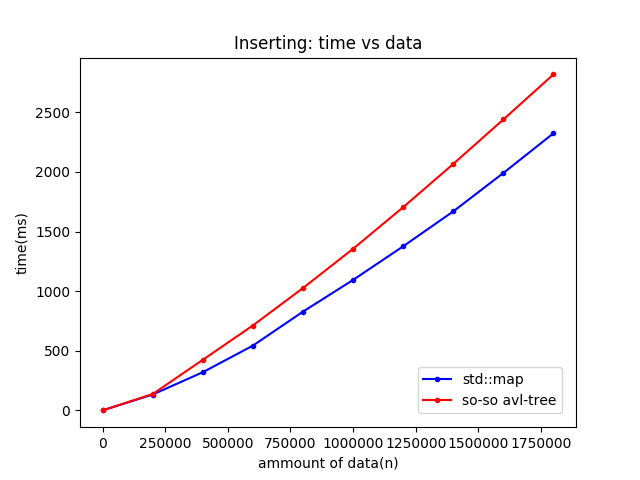
\includegraphics[width=\linewidth]{insert.png}
	\end{center}
	\begin{center}
		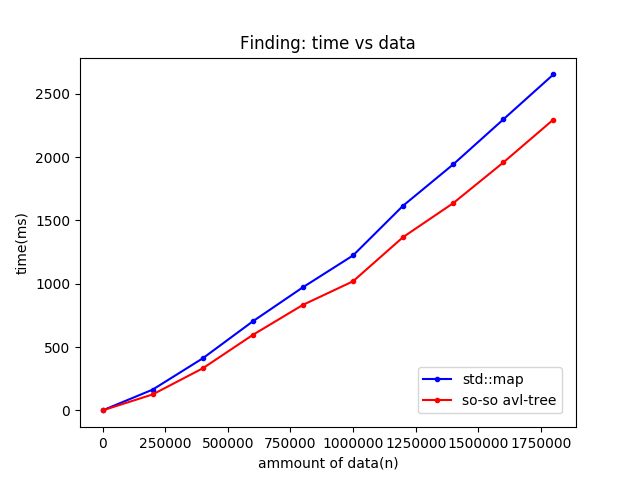
\includegraphics[width=\linewidth]{find.png}
	\end{center}
	
	\begin{center}
		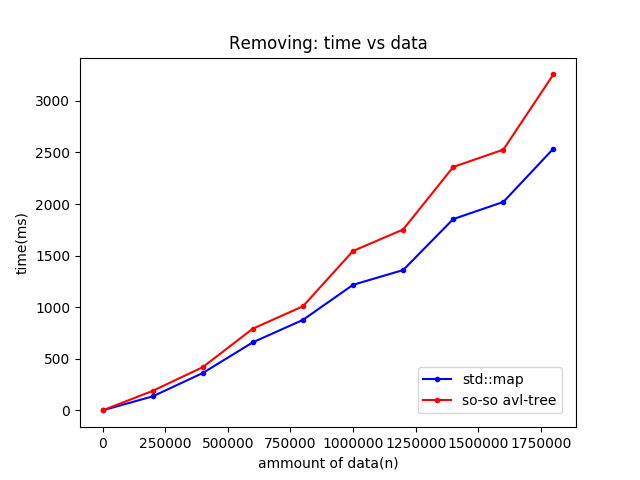
\includegraphics[width=\linewidth]{remove.png}
	\end{center}
	
	Не логарифмическая зависимость на графиках, по моему мнению, получается из-за довольно частых выделений/освобождений памяти на кучи, а это, как известно, не дешевая в плане времени операция.
	К тому же графики имеют очень похожую форму, что говорит об асимптотически одинаковой скорости роста времени выполнения операций. А уж в \verb|stl| сомневаться не приходится.
	
	\subsection*{Недочёты}
	
	Программа работает не так быстро, как хотелось бы, хотя и прошла тестирование на чекере.
	
	\subsection*{Выводы}
	
	Данная стркутура данных может быть применена как вспомогательная для решения большей задачи, например, в качестве словаря, множества, мультимножества(с доработками) и подобных этим абстрактным типам данных. Так же, весьма вероятно, в реализации простейших БД.
	
	Первый раз реализовывать данную структуру было довольно сложно. Возможно, при повторном написании, получится сделать это быстрее и алгоритм получится оптимальнее.
	
	Основные проблемы при написании возникли при реализации удаления из AVL-дерева из-за неполного понимания. Почему-то думалось, что балансировать нужно только дерево-родитель удаляемого узла, а, как оказалось, это не так. 
	
\end{document}
